%\documentclass[a4paper,14pt, unknownkeysallowed]{extreport}
%\documentclass[a4paper,14pt, unknownkeysallowed]{extreport}
\documentclass[a4paper,14pt,unknownkeysallowed]{extreport}

\usepackage{cmap} % Улучшенный поиск русских слов в полученном pdf-файле
\usepackage[T2A]{fontenc} % Поддержка русских букв
\usepackage[utf8x]{inputenc} % Кодировка utf8
\usepackage[english,russian]{babel} % Языки: русский, английский
\usepackage{enumitem}


\usepackage{threeparttable}

\usepackage[14pt]{extsizes}

\usepackage{caption}
\captionsetup{labelsep=endash}  
\captionsetup[figure]{name={Рисунок}}

% \usepackage{ctable}
% \captionsetup[table]{justification=raggedleft,singlelinecheck=off}

\usepackage{amsmath}

\usepackage{geometry}

\usepackage{svg}

\geometry{left=30mm}
\geometry{right=10mm}
\geometry{top=20mm}
\geometry{bottom=20mm}

\usepackage{titlesec}
\titleformat{\section}
	{\normalsize\bfseries}
	{\thesection}
	{1em}{}
\titlespacing*{\chapter}{0pt}{-30pt}{8pt}
\titlespacing*{\section}{\parindent}{*4}{*4}
\titlespacing*{\subsection}{\parindent}{*4}{*4}

\usepackage{setspace}
\onehalfspacing% Полуторный интервал

\frenchspacing
\usepackage{indentfirst} % Красная строка

\usepackage{titlesec}
\titleformat{\chapter}{\LARGE\bfseries}{\thechapter}{20pt}{\LARGE\bfseries}
\titleformat{\section}{\Large\bfseries}{\thesection}{20pt}{\Large\bfseries}

\usepackage{multirow}
\usepackage{listings}
\usepackage{xcolor}

% Для листинга кода:
\lstset{%
	language=c++,   					% выбор языка для подсветки	
	basicstyle=\small\sffamily,			% размер и начертание шрифта для подсветки кода
	numbers=left,						% где поставить нумерацию строк (слева\справа)
	numberstyle=\tiny,		     		% размер шрифта для номеров строк
	stepnumber=1,						% размер шага между двумя номерами строк
	numbersep=5pt,						% как далеко отстоят номера строк от подсвечиваемого кода
	frame=single,						% рисовать рамку вокруг кода
	tabsize=4,							% размер табуляции по умолчанию равен 4 пробелам
	captionpos=t,						% позиция заголовка вверху [t] или внизу [b]
	breaklines=true,					
	breakatwhitespace=true,				% переносить строки только если есть пробел
	backgroundcolor=\color{white},
	basicstyle=\footnotesize\ttfamily,
	keywordstyle=\color{blue},
	stringstyle=\color{red},
	commentstyle=\color{gray}
	showspaces=false,
    showstringspaces=false
}



\usepackage{pgfplots}
\usetikzlibrary{datavisualization}
\usetikzlibrary{datavisualization.formats.functions}




\usepackage{graphicx}
\graphicspath{ {../images/} }
\newcommand{\img}[3] {
	\begin{figure}[h!]
		\center{\includegraphics[height=#1]{img/#2}}
		\caption{#3}
		\label{img:#2}
	\end{figure}
}


\usepackage[justification=centering]{caption} % Настройка подписей float объектов

\usepackage[unicode,pdftex]{hyperref} % Ссылки в pdf
\hypersetup{hidelinks}

\usepackage{csvsimple}

\newcommand{\code}[1]{\texttt{#1}}

\usepackage{longtable}

\usepackage{array}
\usepackage{booktabs}
\usepackage{floatrow}
\usepackage{ulem}


\floatsetup[longtable]{LTcapwidth=table}

\def\UrlBreaks{\do\/\do-\do\_}

\makeatletter
\renewcommand*\l@chapter[2]{%
  \ifnum \c@tocdepth >\m@ne
    \addpenalty{-\@highpenalty}%
    \vskip 1.0em \@plus\p@
    \setlength\@tempdima{1.5em}%
    \begingroup
      \parindent \z@ \rightskip \@pnumwidth
      \parfillskip -\@pnumwidth
      \leavevmode \bfseries
      \advance\leftskip\@tempdima
      \hskip -\leftskip
      #1\nobreak\normalfont\leaders\hbox{$\m@th
        \mkern \@dotsep mu\hbox{.}\mkern \@dotsep
        mu$}\hfill\nobreak\hb@xt@\@pnumwidth{\hss #2}\par
      \penalty\@highpenalty
    \endgroup
  \fi}
\makeatother

%packages for  title
\renewcommand{\underset}[2]{\ensuremath{\mathop{\mbox{#2}}\limits_{\mbox{\scriptsize #1}}}} % Use \underset in normal environment, not only in math

\usepackage{xparse} % \NewDocumentCommand for creating custom commands

% Write stuff under underlined text
\NewDocumentCommand{\ulinetext}{O{3cm} O{c} m m} % O - optional; m - mandatory
{\underset{#3}{\uline{\makebox[#1][#2]{#4}}}}

% Test bold underline
\NewDocumentCommand{\bolduline}{}{\bgroup\markoverwith
{\rule[-0.5ex]{2pt}{2pt}}\ULon}

% Display numberless sections in toc
\NewDocumentCommand{\snumberless}{m}
{\section*{#1}\addcontentsline{toc}{section}{#1}}

\usepackage{tabularx}

% Make sections also use dotted lines; normal font instead of bold in toc
\usepackage{tocloft}
\renewcommand{\cftsecdotsep}{\cftdotsep}
\renewcommand{\cftsecfont}{\normalfont}
\renewcommand{\cftsecpagefont}{\normalfont}

\begin{document}

\begin{titlepage}
    \begin{center}
        \fontsize{12pt}{12pt}\selectfont

        \fbox
        {
            \begin{minipage}{0.15\textwidth}
                
\includegraphics[width=\linewidth]{images/bmstu.png}
            \end{minipage}
            \hfill

            \vrule
            \hspace{0.2cm}

            \begin{minipage}{0.80\textwidth}\centering\bfseries
                {
                    \linespread{1}\selectfont
                    {Министерство науки и высшего образования Российской Федерации}

                    {Федеральное государственное бюджетное~образовательное~учреждение высшего образования}

                    {<<Московский государственный технический университет имени~Н.~Э.~Баумана (национальный~исследовательский~университет)>>}

                    {(МГТУ им. Н.~Э.~Баумана)}
                }
            \end{minipage}
        }

        \vspace{0.2cm}
        \rule{\linewidth}{3.4pt}

        \begin{flushleft}
            {ФАКУЛЬТЕТ \uline{ИУ <<Информатика, искусственный интеллект и системы управления>> \hfill}}

            \vspace{0.5cm}

            {КАФЕДРА \uline{ИУ7 <<Программное обеспечение ЭВМ и информационные технологии>> \hfill}}
        \end{flushleft}

        % \vspace{1cm}

        {
            \Large{\textbf{\bolduline{ОТЧЕТ ПО ПРОИЗВОДСТВЕННОЙ ПРАКТИКЕ}}}

            \vspace{0.5cm}
        }

        \vspace{0.5cm}

        % \setstretch{1.5}
        % \begin{tabular}{p{\textwidth}}
        %     \uline
        %     {
        %         Разработка программы для моделирования столкновений объектов
        %         в виртуальном пространстве. \hfill
        %     }
        %     \rule{\linewidth}{0.4pt}
        % \end{tabular}

        \fontsize{14pt}{14pt}\selectfont

        \begin{flushleft}
            {Студент \uline{Разин Андрей Валерьевич \hfill}}

            \vspace{0.5cm}

            {Группа \uline{ИУ7-44Б \hfill}}

            \vspace{0.5cm}

            {Тип практики \uline{Технологическая \hfill}}

            \vspace{0.5cm}

            % {Название предприятия \uline{\textcolor{red}{\textbf{\Huge ???}} \hfill}}
            {Название предприятия \uline{НУК ИУ МГТУ им. Н. Э. Баумана\hfill}}
        \end{flushleft}

        \vfill

        \begin{flushleft}
            {Студент} \hfill
            \underset{(Подпись, дата)}{\uline{\makebox[3cm][c]{}}}
            \underset{\hfill (И. О. Фамилия)}{\uline{\makebox[4cm][r]{А. В. Разин}}}
            
            \vspace{1.0cm}

            {Руководитель практики} \hfill
            \underset{(Подпись, дата)}{\uline{\makebox[3cm][c]{}}}
            % \underset{\hfill (И. О. Фамилия)}{\uline{\makebox[4cm][r]{\textcolor{red}{\textbf{\Huge ???}}}}}
            \underset{\hfill (И. О. Фамилия)}{\uline{\makebox[4cm][r]{А. В. Куров}}}
            % \underset{\hfill (И. О. Фамилия)}{\uline{\makebox[4cm][r]{}}}

            \vspace{1.0cm}

            {Оценка \ulinetext{}{}} % \uline{\hfill}}

            \vspace{1.0cm}
        \end{flushleft}

        \the\year\ г.

    \end{center}
\end{titlepage}

\thispagestyle{empty} %Удаление нумерации 


\thispagestyle{empty}

\fontsize{12pt}{12pt}\selectfont
\begin{center}
    % \fbox
    {
        % \begin{minipage}{0.15\textwidth}
        %     \includegraphics[width=\linewidth]{img/bmstu_logo.jpg}
        % \end{minipage}
        % \hfill

        % \vrule
        % \hspace{0.2cm}

        \begin{minipage}{0.99\textwidth}\centering\bfseries
            {
                \linespread{1}\selectfont
                {Министерство науки и высшего образования Российской Федерации}

                {Федеральное государственное бюджетное~образовательное~учреждение высшего образования}

                {<<Московский государственный технический университет имени~Н.~Э.~Баумана (национальный~исследовательский~университет)>>}

                {(МГТУ им. Н.~Э.~Баумана)}
            }
        \end{minipage}
    }

    \vspace{0.2cm}

    \rule{\linewidth}{3.4pt}
\end{center}

\fontsize{11pt}{11pt}\selectfont
\begin{flushright}
    \begin{minipage}{0.4\textwidth}\raggedleft

        УТВЕРЖДАЮ \hspace{2.5cm}

        % Заведующий кафедрой~\ulinetext[2cm]{(Индекс)}{ИУ7}
        Заведующий кафедрой~\ulinetext[2cm]{}{ИУ7}

        \vspace{0.3cm}

        % \ulinetext{}{} \ulinetext{\hfill (И. О. Фамилия)}{И. В. Рудаков}
        \ulinetext{}{} \ulinetext{}{И. В. Рудаков}

        \vspace{0.3cm}

        << \ulinetext[1cm]{}{} >> \ulinetext{}{} \the\year \ г.
    \end{minipage}
\end{flushright}

\begin{center}\linespread{1}\selectfont
    \Large{\textbf{ЗАДАНИЕ}}

    \large{\textbf{на прохождение производственной практики}}

    \large{\ulinetext[0.7\textwidth]{Тип практики}{Технологическая}}
\end{center}

\fontsize{14pt}{14pt}\selectfont

\noindent Студент \uline{\hfill Разин Андрей Валерьевич \hfill} \ulinetext[1cm]{№ курса}{2} курса группы \ulinetext{индекс группы}{ИУ7-44Б}

\vspace{0.3cm}

\noindent в период с \ulinetext[1cm]{}{01}.\ulinetext[1cm]{}{07}.2023 г. по \ulinetext[1cm]{}{21}.\ulinetext[1cm]{}{07}.2023 г.

\vspace{0.3cm}

\noindent \textit{Предприятие:} \uline{\hfill НУК ИУ МГТУ им. Н. Э. Баумана \hfill}

\vspace{0.3cm}

% \noindent \textit{Подразделение:} \uline{\hfill}

% \vspace{0.3cm}

% \noindent \textit{Руководитель практики от предприятия (наставник):}

% \noindent \ulinetext[\linewidth]{(Фамилия Имя Отчество полностью, должность)}{\hfill}

% \vspace{0.3cm}

\noindent \textit{Руководитель практики от кафедры:}

\noindent \ulinetext[\linewidth]{(Фамилия Имя Отчество полностью)
% , должность)
}{\hfill Куров Андрей Владимирович \hfill}

\vspace{0.3cm}

\noindent \textit{Задание:}

Разработать программное обеспеченье с пользовательским интерфейсом для моделирования отражения от геометрических тел. 
Рассматриваемые тела будут являться трехмерными примитивами: шар, куб, цилиндр, конус, имеющими настраиваемые параметры отражения (коэффициент отражения, тип отражения). 
Должна быть возможность изменения положения источника света и перемещения камеры. 
Также должна быть реализована возможность изменять интенсивность источника света. 
Интерфейс должен позволить изменять параметры примитивов: должна быть возможность изменения цвета примитивов и положения в пространстве (перемещение и поворот).


\vfill

\noindent Дата выдачи задания <<\ulinetext[1cm]{}{01}>>\ulinetext{}{июля} 2023 г.

\vspace{1cm}

% \noindent Руководитель практики от предприятия \hfill \ulinetext[2cm]{}{}/\ulinetext[4cm]{}{}/

% \vspace{0.3cm}

\noindent Руководитель практики от кафедры \hfill \ulinetext[2cm]{}{}/\ulinetext[4cm]{}{\hfill Куров А. В. \hfill}/

\vspace{0.3cm}

\noindent Студент \hfill \ulinetext[2cm]{}{}/\ulinetext[4cm]{}{\hfill Разин А. В. \hfill}/

\vfill

% \noindent Дата выдачи задания << \uline{\hspace{0.5cm}} >> \uline{\hspace{2cm}} \the\year \ г.
\thispagestyle{empty} 





\renewcommand{\contentsname}{Содержание} 
\tableofcontents


\setcounter{page}{2}
\chapter{Введение}

Компьютерная графика играет важнейшую роль в современной жизни. 
Она позволяет нам видеть различные задачи в совершенно новом свете, а также создавать и исследовать визуально привлекательные и живые изображения.
С ее помощью мы можем представлять друг другу информацию с помощью цветного и анимированного содержимого. 
Получение качественного изображения необходимо во многих областях, включая медицину, искусство и игры.
Особенно важной становится задача генерации реалистичного изображения, с развитием технологий люди привыкают к все более
правдоподобной картинке. Чаще всего люди подмечают нереалистичность изображения при наблюдении света: его отражения и преломления.


Целью данной работы является разработка программного обеспечения, моделирующего отражения от геометрических тел.Для достижения поставленной цели требуется
решить следующие задачи:
\begin{enumerate}
	\item Формализировать представление объектов сцены и описать их
	\item Проанализировать алгоритмы построения реалистичных изображений и теней
	\item Выбрать наилучшие алгоритмы для достижения цели  из рассмотренных
	\item Проанализировать полученную  модель взаимодействия света с объектами
	\item Выбрать програмные средства для реализации модели
	\item Реализовать полученную модель
	\item Создать интерфейс
	\item Провести замеры временных характеристик полученной модели
\end{enumerate}





\chapter{Аналитическая часть}
\section[Формализация объектов синтезируемой сцены]{Формализация объектов синтезируемой сцены}
\label{sec:obj_formalasation}
На визуализируемой сцене могут находится следующие объекты:
\begin{enumerate}
	\item \textbf{Точечный источник света}
	Данный источник света излучает свет во всех направлениях, интенсивность света убывает при отдалении от источника.
	Источник характеризуется:
	\begin{enumerate}[label*=\arabic*.]
		\item Положением в пространстве
		\item Интенсивностью
	\end{enumerate}
	При расчете отражений будет использоваться интенсивность источника,для расчета интенсивности пикселей. Цвет свечения будет описываться через значения RGB.
	%(TODO - в случае если останется время на физически верный расчет интенсивности то добавить постоянный,линейный и квадратичный коэффициенты)
	\item \textbf{Объекты сцены}
	
	Объектами сцены являются трехмерные примитивы:
	\begin{enumerate}[label*=\arabic*.]
		\item \textbf{Шар}
		
		Для описания шара потребуется:
		\begin{enumerate}[label*=\arabic*.]
			\item Радиус
			\item Координаты центра
		\end{enumerate}
		\item  \textbf{Куб}
		
		Для описания куба потребуется:
		\begin{enumerate}[label*=\arabic*.]
			\item Координаты центра
			\item Координаты вершин относительно центра
			\item Индексы соединенных вершин(Ребра)
		\end{enumerate}
		\item  \textbf{Конус}
		
		Для описания конуса потребуется:
		\begin{enumerate}[label*=\arabic*.]
			\item Координаты центра окружности основания конуса
			\item Радиус основания конуса
			\item Координата верхней точки конуса
		\end{enumerate}
		\item  \textbf{Цилиндр}
		
		Для описания цилиндра потребуется:
		\begin{enumerate}[label*=\arabic*.]
			\item Координаты центра нижнего основания цилиндра
			\item Координата центра верхнего основания конуса
			\item Радиус цилиндра
		\end{enumerate}
		Заметим, что каждый из примитивов также должен описываться своим цветом в формате RGB, а также
		коэффициентами рассеянного, диффузного,зеркального отражения
		%TODO::Некое наитие что проще все свести к полигонам и хранить все в *.obj
	\end{enumerate}

	\item \textbf{Камера}
	
	В данном случае камера может описываться:
	\begin{enumerate}[label*=\arabic*.]
		\item Координатами своего положения
		\item Вектором направления взгляда
		\item Правым вектором пространства камеры
		\item Верхним вектором пространства камеры
	\end{enumerate}
	
\end{enumerate}

\section[Анализ моделей отражения]{Анализ моделей отражения}
\label{sec:reflection_models}
Свет отраженный от объекта может быть диффузным и зеркальным.
Диффузное отражение происходит, когда свет поглощается поверхностью, а затем вновь испускается, в данном случае
отражение равномерно рассеивается по всем направлениям и положение наблюдателя не имеет значения.Зеркальное отражение
происходит от внешней поверхности объекта, оно является направленным и зависит от положения наблюдателя.
Так как отражение происходит от внешней части объекта ,то отраженный свет сохраняет свойства падающего, например в случае если белый свет отражается
от красного тела, отраженный свет также будет нести в себе часть красного цвета.
Для расчета интенсивности света данных отражений существует несколько моделей:
\begin{enumerate}
	\item Модель Ламберта
	\item Модель Фонга \cite{Rodgers}
\end{enumerate}

\subsection{Модель Ламберта}
В данной модели рассматривается диффузная составляющая отражения.

\begin{figure}[h]
	\centering
	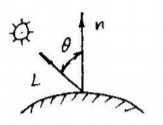
\includegraphics{lambert_model}
	\caption{Модель ламберта}
	\label{fig:lambert_model}
\end{figure}

Считается, что интенсивность отраженного света
пропорциональна косинусу угла между направлением света и нормалью к поверхности:
\begin{equation} 
	I = k_aI_a + I_lk_l\cos\theta \quad 0 \leq \theta \leq \pi/2.
	\label{eq:lambert_model}
\end{equation}
В  формуле~\ref{eq:lambert_model}:
\begin{enumerate}
	\item $k_a,k_d$ - коэффициенты рассеянного, диффузного отражения соответственно
	\item $I_a,I_l$ - интенсивность рассеянного и диффузного отражения 
	\item $theta$ - угол между нормалью к поверхности и направлением света
\end{enumerate}
Заметим что значения приведенных коэффициентов лежат на отрезке от 0 до 1.

Однако интенсивность света должна убывать с увеличением расстояния от источника до объекта, эмпирически было выведено следующее соотношение:
\begin{equation} 
	I = k_aI_a + \frac{I_lk_l\cos\theta}{d + K}.
	\label{eq:lambert_model_space}
\end{equation}
В данном случае добавлены $d,K$, в случае если точка наблюдения на бесконечности, то $d$ - определяется положением объекта,
ближайшего к точке наблюдения, то есть он будет освещаться с максимальной интенсивностью источника, а дальние объекты - с уменьшенной.
$K$ в данном случае - произвольная постоянная. \cite{Rodgers}


\subsection{Модель Фонга}
Данная модель также учитывает зеркальную составляющую отражения
\begin{figure}[h]
	\centering
	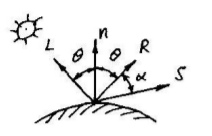
\includegraphics{phong_model}
	\caption{Расчет зеркальной составляющей отражения}
	\label{fig:phong_model}
\end{figure}
\newline
Зеркальная составляющая отражения имеет следующий вид:
\begin{equation} 
	I_s = I_l\omega(i,\lambda)\cos^n \alpha.
	\label{eq:phong_model}
\end{equation}

В формуле~\ref{eq:phong_model} символы соответственно означают:
\begin{enumerate} 
	\item $\omega(i,\lambda)$ - кривая отражения,показывающая отношение зеркально отраженного света к падающему, как функцию угла падения $i$ и длинны волны $\lambda$
	\item $\alpha$ - угол между отраженным лучом и вектором, проведенным из точки падения луча в точку наблюдения 
	\item $n$ - степень, аппроксимирующая пространственное распределение отраженного света
	\item $I_l$ - интенсивность падающего луча
\end{enumerate}
Функция $\omega(i,\lambda)$ сложна, так что ее заменяют константой $k_s$, получаемой экспериментально.


Таким образом формула принимает следующий вид:
\begin{equation} 
	I = k_aI_a + k_dI_{l}(\hat{n} \cdot \hat{L}) + k_s  I_{l}(\hat{S} \cdot \hat{R})^n.
\end{equation}
В данном случае косинусы вычисляются с помощью скалярного произведения нормированных векторов:
\begin{enumerate}
	\item $\hat{n}$ - вектор нормали поверхности в точке падения
	\item $\hat{L}$ - вектор падающего луча
	\item $\hat{S}$ - вектор наблюдения
	\item $\hat{R}$ - вектор отражения
\end{enumerate}
Символ $\hat{}$ означает, что данный вектор нормированный.\cite{Rodgers}




\subsection{Выбор модели отражения}
Данные модели описывают простую (локальную) модель освещения,то есть модель освещения в которой учитывается свет, попадающий в рассматриваемую точку от источника света.
Для получения отражений стоит использовать глобальную модель освещения, в которой также учитывается интенсивность света, отраженного от других поверхностей, пример описания глобальной модели излучения можно найти в секции~\ref{sec:ray_tracing}.
Заметим, что глобальная модель в случае алгоритма Уиттеда освещения использует идею модели Фонга (см.~\ref{eq:intensivity}).


\section{Анализ алгоритмов закраски}
Для сглаживания и добавления реализма изображениям  необходимо использовать алгоритмы закраски.
В данном случае будут рассмотрены 2 алгоритма закраски:
\begin{enumerate}
	\item Простая закраска
	\item Закраска методом Гуро
	\item Закраска методом Фонга
\end{enumerate}

\subsection{Простая закраска}
В случае использования простой закраски считается,что и источник света и наблюдатель находятся в бесконечности,
так что диффузная составляющая одинакова (она зависит от угла падения), вектор наблюдения также будет для всех точек одинаковым, то есть зеркальная составляющая
также не будет изменяться (см.~\ref{sec:reflection_models}). 
Таким образом данный алгоритм является быстрым, однако в случае, если закрашиваемая грань является результатом аппроксимации тела, 
будет заметен резкий переход между интенсивностями. \cite{Rodgers}


\subsection{Закраска методом Гуро}
В случае использования метода Гуро можно получить сглаженное изображение, для этого сначала определяется интенсивность вершин многоугольника, а
затем с помощью билинейной интерполяции вычисляется интенсивность каждого пиксела на сканирующей строке.

\begin{figure}[H]
	\centering
	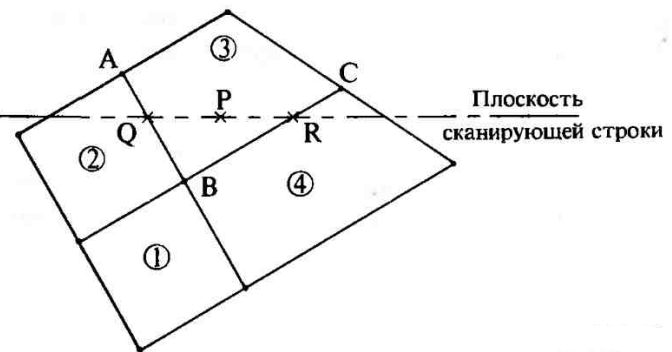
\includegraphics{guro}
	\caption{Пример полигональной поверхности}
	\label{fig:guro_polygon}
\end{figure} 

Например, рассмотрим участок полигональной поверхности на рисунке~\ref{fig:guro_polygon}.
Значение интенсивности в точке P
определяется линейной интерполяции значений интенсивностей в точках Q и R.
Для получения интенсивности в точке Q можно провести линейную интерполяцию интенсивности в вершинах A и B (см. формула~\ref{eq:guro_inter_1}).
\begin{equation} 
	I_Q = uI_A+(1-u)*I_B  \quad 0 \leq u \leq 1, t = \frac{AQ}{AB}.
	\label{eq:guro_inter_1}
\end{equation}
Таким же образом рассчитывается интенсивность в точке B, после чего интерполяция используется еще раз, для поиска значения интенсивности в точке P 
(см. формула~\ref{eq:guro_inter_2}). \cite{Rodgers}
\begin{equation} 
	I_P = tI_Q+(1-t)*I_R  \quad 0 \leq t \leq 1, t = \frac{QP}{QR}.
	\label{eq:guro_inter_2}
\end{equation}

\textbf{Недостатки метода:}
\begin{enumerate}
	\item Появление полос Маха 
	\item Не учитывает кривизны поверхности (случай, если нормали поверхностей одинаково ориентированы)
\end{enumerate}

\textbf{Достоинства метода:}
\begin{enumerate}
	\item Получение сглаженного изображения
	\item Небольшие трудозатраты
\end{enumerate}


\subsection{Закраска методом Фонга}
Закраска Фонга требует больших вычислительных затрат, однако она решает множество проблем метода Гуро.В данном методе вместо интерполяции интенсивностей света,
производится интерполяция вектора нормали.Таким образом учитывается кривизна поверхности.
В случае картинки~\ref{fig:guro_polygon}, нормали в соответствующих точках рассчитывалась бы формулами~\ref{eq:phong_shading}. \cite{Rodgers}
\begin{equation}
	\label{eq:phong_shading}
	\begin{aligned}
	n_Q = un_A + (1-u)n_B  \quad 0 \leq u \leq 1 \\
	n_R = wn_B + (1-w)n_C  \quad 0 \leq w \leq 1 \\
	n_P = tn_Q + (1-t)n_R  \quad 0 \leq t \leq 1.
	\end{aligned}
\end{equation}
где
\begin{equation}
	\begin{aligned}
	u = \frac{AQ}{AB} \\\\
	w = \frac{BR}{BC} \\\\
	t = \frac{QP}{QR} 
	\end{aligned}
\end{equation}

\textbf{Недостатки метода:}
\begin{enumerate} 
	\item Высокая трудозатратность алгоритма
\end{enumerate}

\textbf{Достоинства метода:}
\begin{enumerate}
	\item Получение сглаженного изображения
	\item Учет кривизны поверхностей
	\item Улучшенная реалистичность зеркальных бликов (по сравнению с методом Гуро)`'
\end{enumerate}


\subsection{Выбор метода закраски}
На картинах~\ref{fig:shading_compare} и~\ref{fig:reflexion_shading_compare} представлены различные методы закраски. Заметим, что наиболее реалистичным методом закраски является
закраска Фонга, так как она учитывает кривизну тел и лучше визуализирует блики, так что для высокого качества изображения стоит воспользоваться методом Фонга.

\begin{figure}[H]
	\centering
	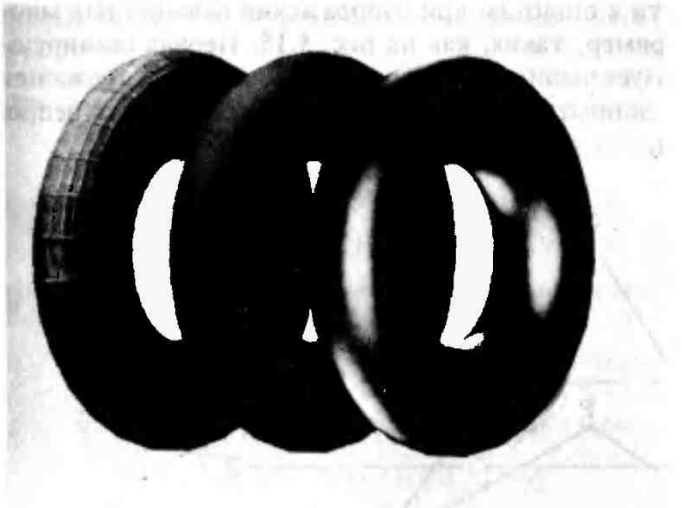
\includegraphics{shading_compare}
	\caption{Сравнение методов закраски: слева - простая, посередине - методом Гуро, справа - методом Фонга}
	\label{fig:shading_compare}
\end{figure}

\begin{figure}[H]
	\centering
	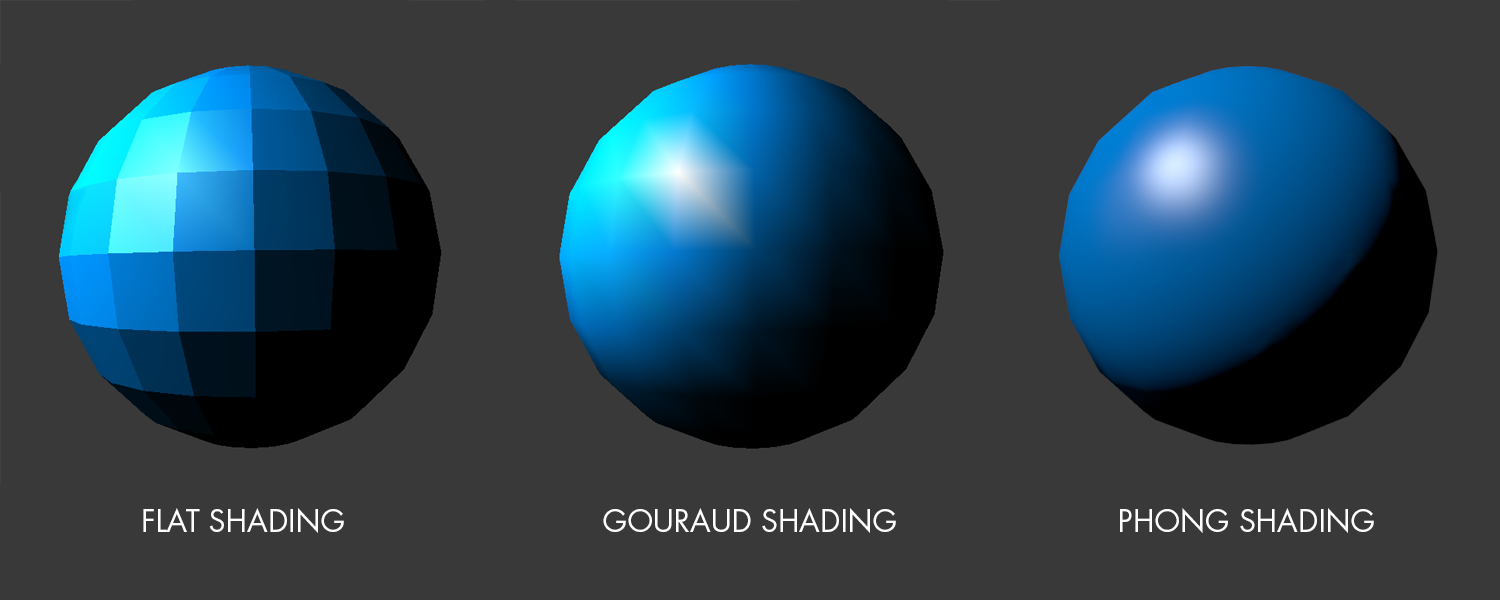
\includegraphics[scale=0.3]{reflexion_shading_compare}
	\caption{Сравнение бликов при различных методах закраски}
	\label{fig:reflexion_shading_compare}
\end{figure}






\section[Анализ алгоритмов создания отражений]{Анализ алгоритмов визуализации}

Для начала рассмотрим пример отражения лучей:

\begin{figure}[H]
	\centering
	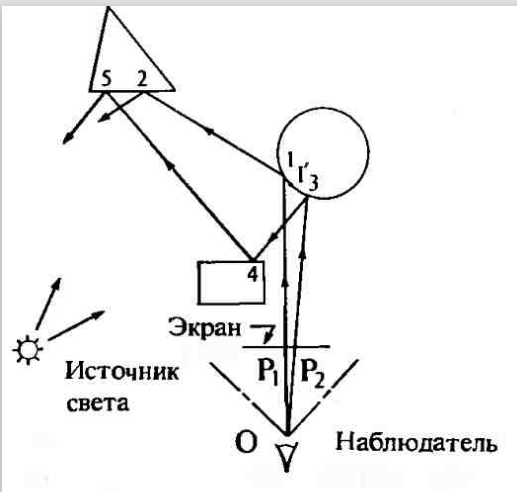
\includegraphics{global_model_light.png}
	\caption{Пример трассировки луча}
	\label{fig:global_model_light}
\end{figure} 

Заметим что на рисунке~\ref{fig:global_model_light}  призма, загороженная от наблюдателя параллелепипедом,становится видимой из-за отражения в сфере.
Точка 5 видима, так как отражается от обратной стороны параллелепипеда в точке 4 к точке 3 на сфере, а затем к наблюдателю.
Таким образом, при создании глобальной модели освещения, алгоритмы , основанные на удалении невидимых поверхностей не будут давать изображения необходимого качества.
Таким образом глобальная модель освещения является частью алгоритмов выделения видимых поверхностей путем трассировки лучей\cite{Rodgers}


При построении реалистичного изображения необходимо с полированными поверхностями необходимо визуализировать отражения света от тел.
Существуют множество подходов для создания реалистичных изображений:
\begin{enumerate}
	\item Трассировка световых лучей (Ray tracing)
	\item Отображения отражений (Reflection mapping)
	\item Трассировка лучей в пространстве изображения(Screen-space reflections)
\end{enumerate}





\subsection{Алгоритм трассировки лучей}
\label{sec:ray_tracing}
\textbf{Основная идея алгоритма - симуляция физического процесса прохождения света} \newline
В реальной жизни объекты являются видимыми, в случае если они отражают свет от источника, после чего данные лучи света попадают в человеческий глаз.Аналогичная идея заложена в данном способе создания изображения - необходимо отследить движение лучей света.
Заметим, что отслеживать путь всех лучей света не стоит, так как это неэффективно, при построении изображения внимание следует уделять объектам видимыми со стороны наблюдателя.
В таком случае можно отслеживать лучи света, исходящие из точки наблюдения, т.~е. производить трассировку лучей в обратном направлении.В нашем случае лучи стоит проводить через центры пикселей изображения,
считается ,что наблюдатель находится на бесконечности, из-за чего все лучи параллельны оси OZ.\cite{Rodgers,modern_ray_tracing}

\begin{figure}[h]
	\centering
	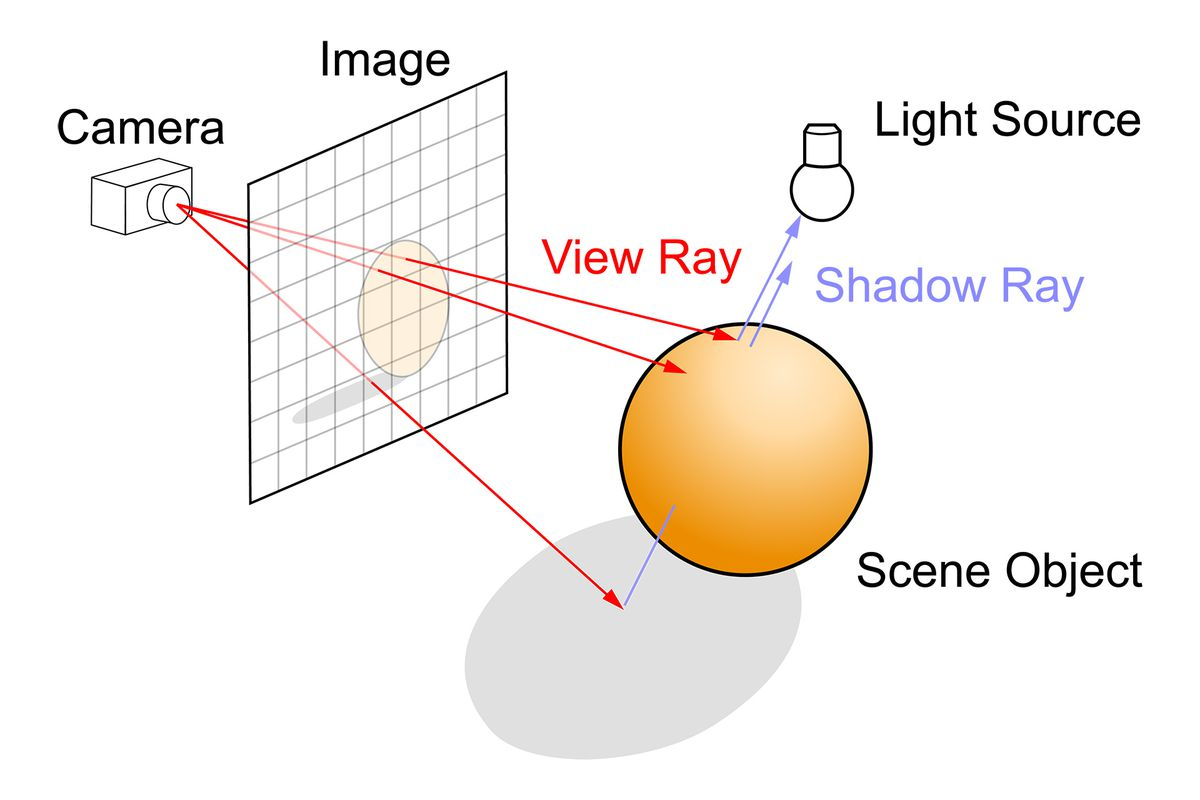
\includegraphics[scale=0.4]{ray_tracing.jpg}
	\caption{Пример трассировки луча}
	\label{fig:alg_ray_tracing}
\end{figure} 

Первые работы принадлежат Уиттеду и Кэю.Алгоритм Уиттеда более общий и часто используется.[Роджерс с.438]
Уиттед пользуется моделью , в которой диффузная и зеркальная составляющие отражения рассчитываются подобно локальной модели (см.~\ref{sec:reflection_models}).
Диффузное отражения одинаково во всех направлениях, так что наибольшую проблему представляет расчет зеркальных отражений.\cite{Rodgers}

\begin{figure}[h]
	\centering
	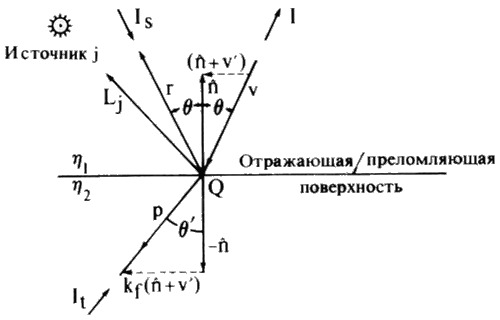
\includegraphics{global_reflections}
	\caption{Расчет зеркального отражения луча в алгоритме Уиттеда}
	\label{fig:global_reflections}
\end{figure} 

На рисунке ~\ref{fig:global_reflections} луч \textbf{V} падает на поверхность в точку \textbf{Q}, после чего отражается в направлении \textbf{r} и преломляется
в направлении \textbf{p}.
В данном случае:
\begin{enumerate}
	\item $I_t$ - интенсивность света, проходящего по преломленному лучу \textbf{p}.
	\item $\eta$ - показатели преломления сред(влияют на направление преломленного луча)
	\item $\hat{S}$,$\hat{R}$ - полученные вектора наблюдения и отражения
	\item $\hat{L_j}$ - Вектор к источнику света $j$

\end{enumerate}

Тогда наблюдаемая интенсивность \textbf{I} выражается формулой:
\begin{equation} 
	I = k_aI_a + k_d \sum_{j} I_{l_j}(\hat{n} \cdot \hat{L_j}) + k_s \sum_{j} I_{l_j}(\hat{S} \cdot \hat{R_j})^n + k_sI_s + k_tI_t.
	\label{eq:intensivity}
\end{equation}

В формуле~\ref{eq:intensivity} соответственно означают:
\begin{enumerate}
	\item $k_a,k_d,k_s$ - коэффициенты рассеянного, диффузного,зеркального отражения соответственно
	\item $k_t$ - коэффициент пропускания
	\item $n$ - степень пространственного распределения Фонга
\end{enumerate}
В данном случае знак $ \hat{} $  означает что данный вектор нормализован.
Значения коэффициентов определяются внешней средой,свойствами материала объектов и длинной волн света
Таким образом возможно посчитать интенсивность света для отраженной и преломленной части луча.
После чего полученные вычисления необходимо выполнить еще раз для отраженного и преломленного луча и т.~д.
, а также сложить полученные интенсивности.
Теоретически свет может отражаться бесконечно, так что стоит ограничить число рассматриваемых отражений либо определенным числом,
либо не рассматривать лучи с интенсивностью меньше определенного значения
Таким образом данный алгоритм имеет асимптотику $O(N \cdot C \cdot 2^{K})$ , где \textbf{N} - количество тел,\textbf{C} - количество испускаемых лучей,
\textbf{K} - количество рассматриваемых отражений света. \cite{Rodgers}



\textbf{Достоинства алгоритма}:
\begin{enumerate}
	\item Создание реалистичных изображений \cite{Rodgers,modern_ray_tracing,SSR}
	\item Возможность наблюдения физических явлений, так как алгоритм симулирует поведение света в реальной жизни \cite{Rodgers,modern_ray_tracing,SSR}
\end{enumerate}


\textbf{Недостатки алгоритма}:
\begin{enumerate}
	\item Время работы \cite{Rodgers,modern_ray_tracing,SSR}
	\item Количество требуемой памяти, так как в памяти необходимо хранить все отраженные и преломленные лучи, полученные при предыдущих расчетах \cite{Rodgers,modern_ray_tracing,SSR}
\end{enumerate}


\subsection{Трассировка лучей в пространстве изображения}
\textbf{Основная идея алгоритма - симуляция физического процесса прохождения света, рассматривая только видимые объекты} \newline
Обычно при необходимости расчета отражений и теней уже известны объекты, которые находятся на сцене.При использовании SSR(Screen-space reflections),используется информация о имеющихся
объектов из-за чего трудозатраты на создание изображения заметно сокращаются.
Асимптотическая оценка данного алгоритма аналогична асимптотической оценке алгоритма трассировке лучей, однако в данном случае будут анализироваться только видимые объекты.\cite{SSR}

Перед началом алгоритма требуется информация для каждого пикселя:
\begin{enumerate}
	\item Координата Z наиближайшей к наблюдателю поверхности
	\item Нормаль данной поверхности
\end{enumerate}

\begin{figure}[H]
	\centering
	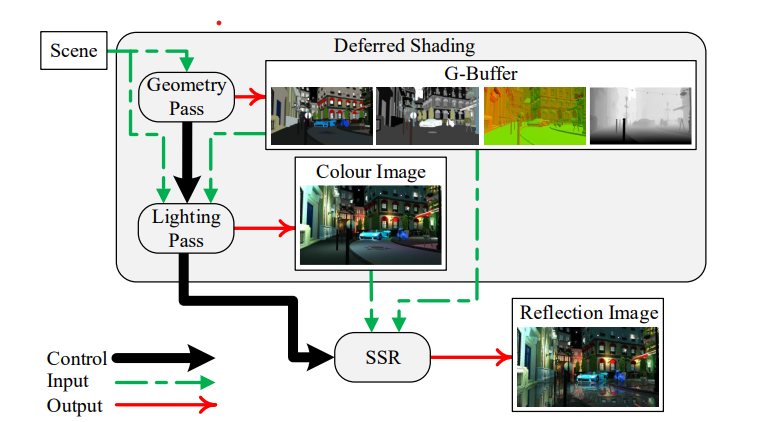
\includegraphics{SSR_data_flow.png}
	\caption{Поток данных при использовании SSR}
	\label{fig:SSR_data_flow}
\end{figure} 

До начала работы самого алгоритма необходимо подготовить данные, что происходит в два этапа:
\begin{enumerate}
	\item Геометрический проход(Geometry pass)
	\item Световой проход(Lightning pass)
\end{enumerate}

На картинке~\ref{fig:SSR_data_flow} используется понятие \textbf{G-buffer}, данный буфер содержит все необходимые данные для начала работы алгоритма,данные для данного буфера
будут получены после геометрического прохода. В общем случае он содержит для каждого пикселя:
\begin{enumerate}
	\item Нормали к видимым поверхностям
	\item Значение z наиближайшей видимой фигуры
	\item Свойства материалов, значимые для трассировки света(коэффициенты диффузного и зеркального отражения)
\end{enumerate}
При световом проходе для каждого пикселя выбираются источники,которые влияют на его интенсивность
Работа SSR аналогична работе алгоритма \textbf{Ray tracing},однако информация о видимых объектах уже получена и будут рассматриваться только они.
Из-за этого,если часть объекта не видима то изображение будет не корректным, как ,например, на картинке~\ref{fig:SSR_fail}.\cite{SSR,reflexion_types}
\begin{figure}[H]
	\centering
	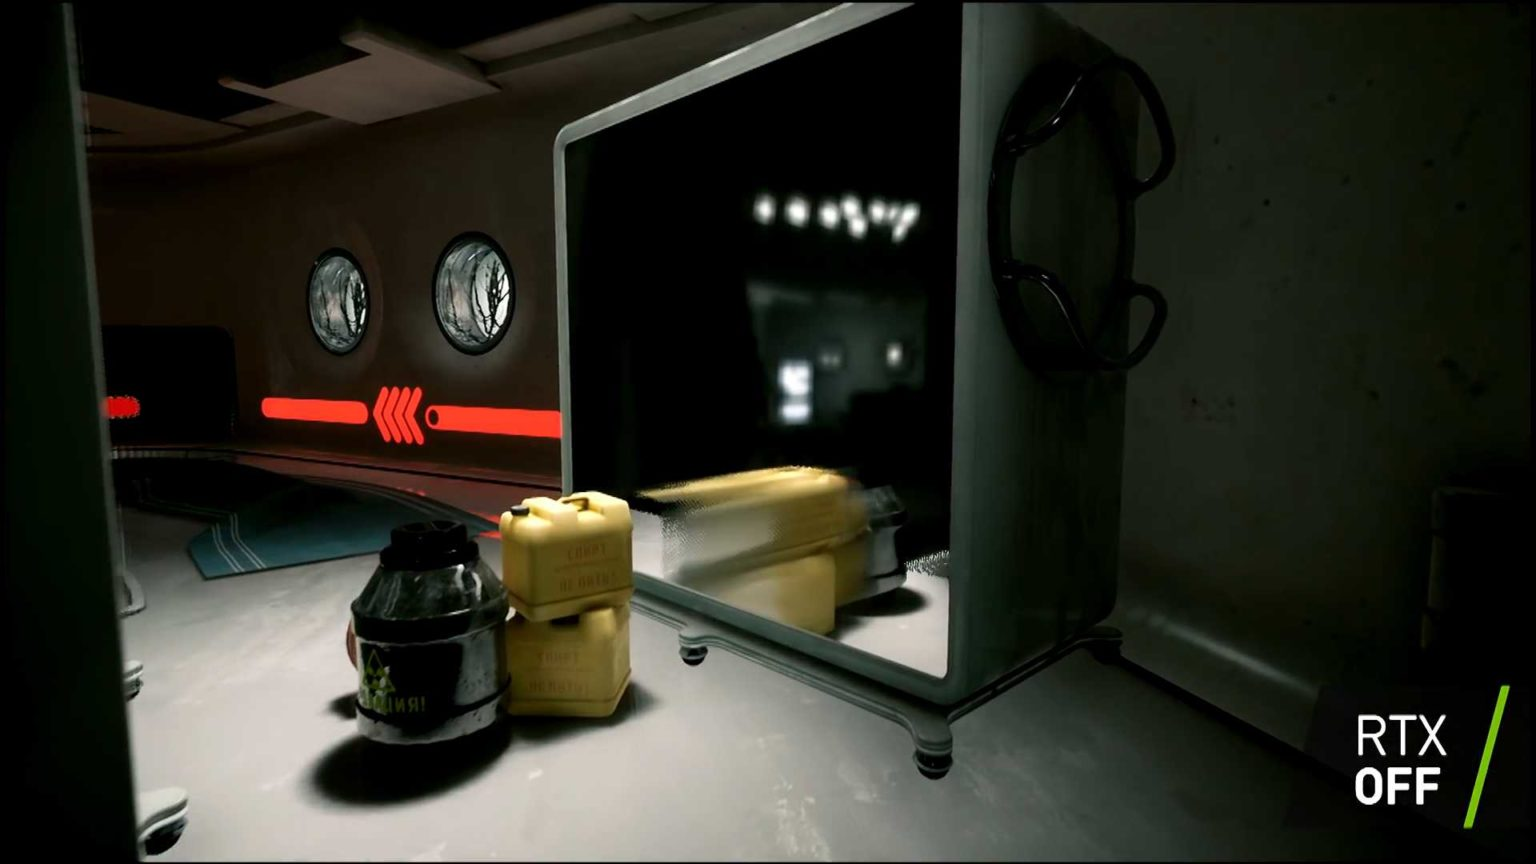
\includegraphics[scale=0.4]{SSR_fail.jpg}
	\caption{Некорректный расчет отражений при использовании SSR}
	\label{fig:SSR_fail}
\end{figure} 

\textbf{Достоинства алгоритма}:
\begin{enumerate}
	\item Меньшее число трудозатрат,чем при использовании алгоритма трассировки лучей \cite{SSR}
\end{enumerate}

\textbf{Недостатки алгоритма}:
\begin{enumerate}
	\item При наличии невидимых для наблюдателя частей объектов в отражении изображение будет некорректным \cite{SSR}
	\item Искаженem Искажение геометрии при генерации изображений \cite{SSR}
\end{enumerate}

\subsection{Отображение отражений}
\textbf{Основная идея - создание текстуры с уже просчитанными отражениями,после чего наложить ее на зеркальный предмет} \newline
Для того чтобы получить текстуру,достаточно предварительно рассчитать изображения в 6 направлениях для необходимого объекта, получив кубическую карту, ее пример представлен на картинке~\ref{fig:cube_maps}.\cite{reflexion_types}
\begin{figure}[h]
	\centering
	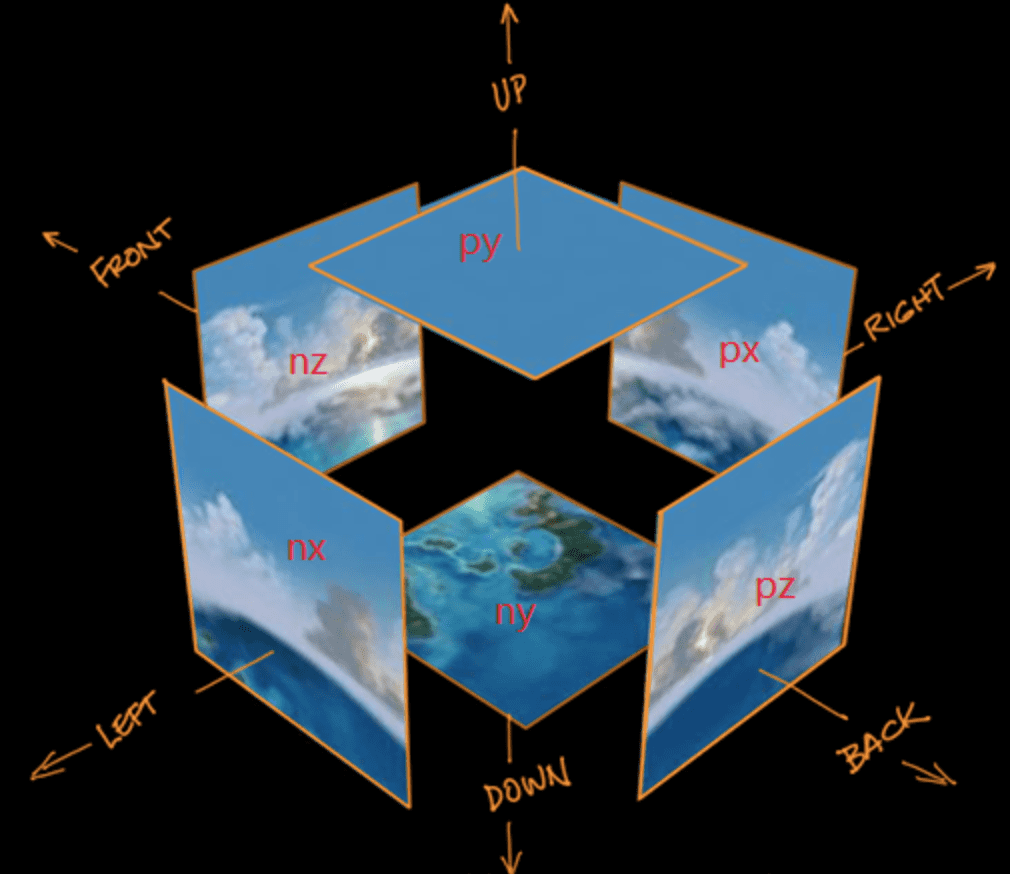
\includegraphics[scale=0.4]{cube_maps}
	\caption{Пример кубической карты(cube maps)}
	\label{fig:cube_maps}
\end{figure}

Например для объекта~\ref{fig:cube_maps_real}, будет получена карта~\ref{fig:cube_maps_real_example}


\begin{figure}[H]
	\centering
	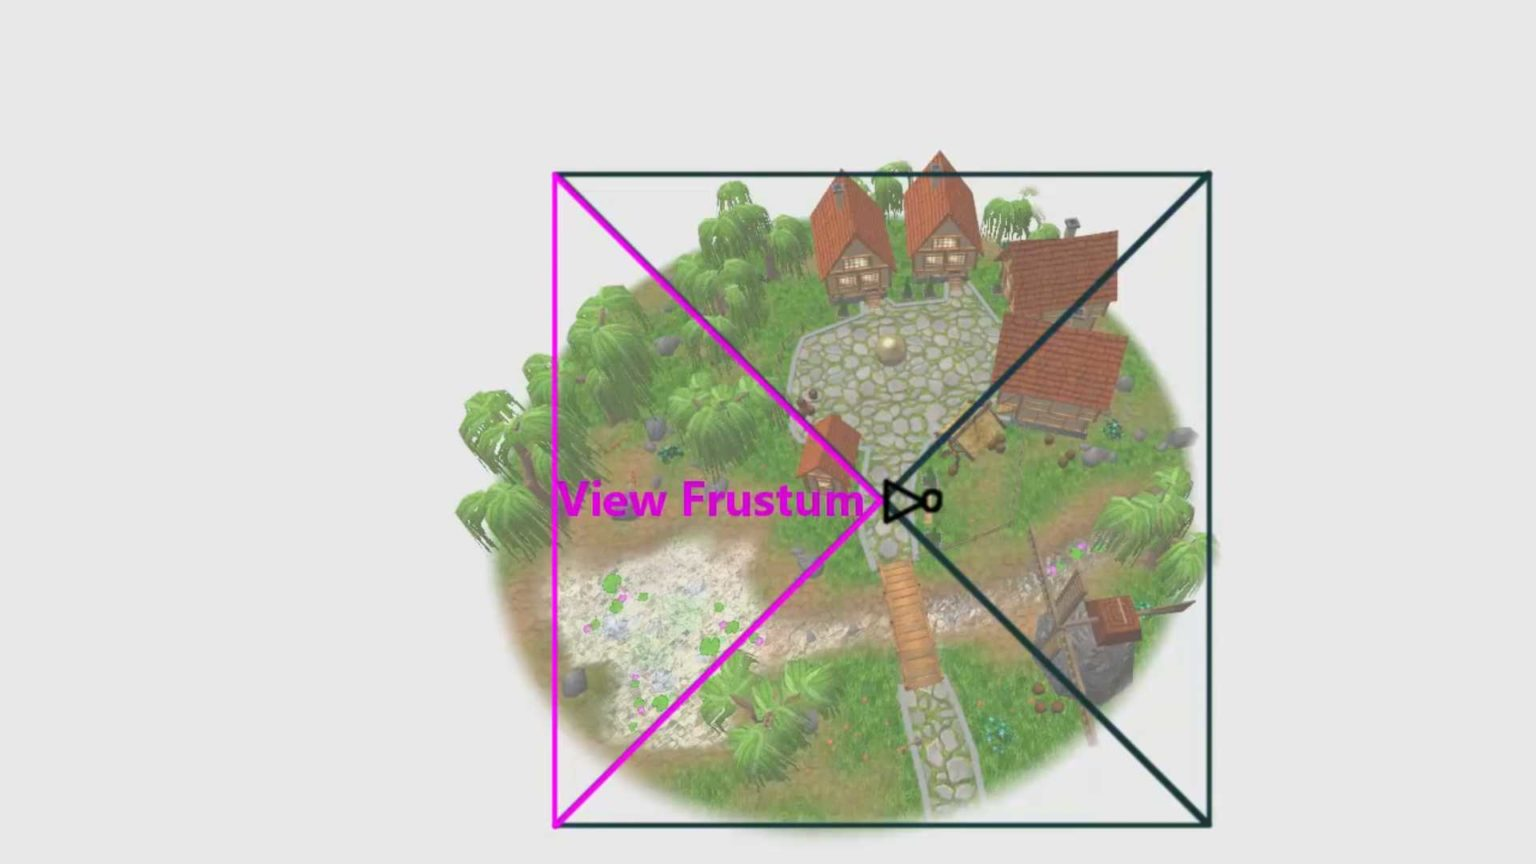
\includegraphics[scale=0.4]{cube_maps_real}
	\caption{Положение объекта для построения карты}
	\label{fig:cube_maps_real}
\end{figure}


\begin{figure}[H]
	\centering
	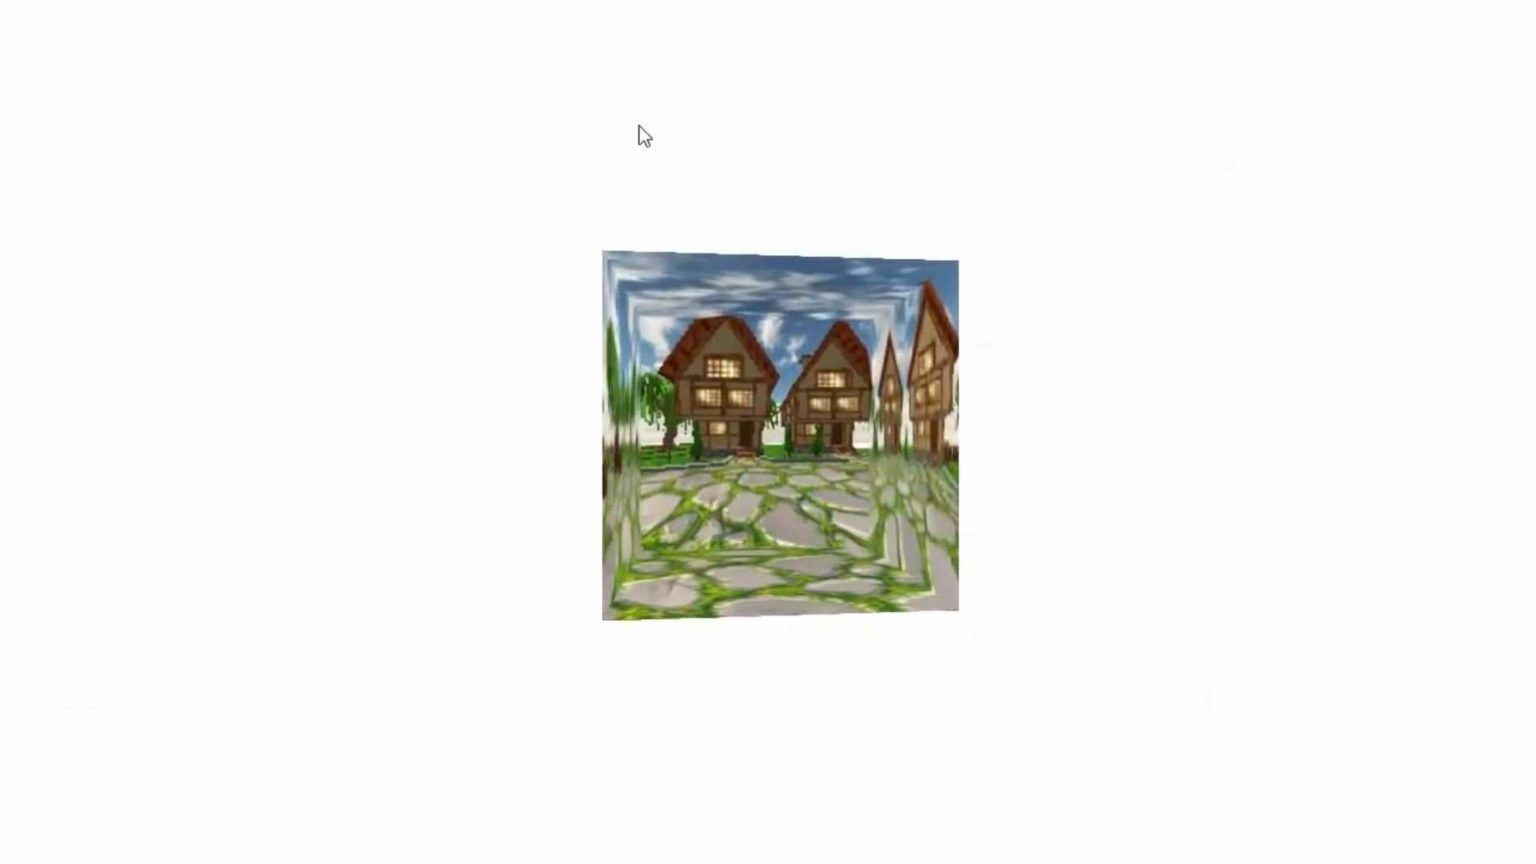
\includegraphics[scale=0.4]{cube_maps_real_example}
	\caption{Полученная кубическая карта}
	\label{fig:cube_maps_real_example}
\end{figure}


Однако динамически обновлять данную текстуру очень трудозатратно (необходимо отрсиовать сцену 6 раз).Асимптотическая оценка зависит от алгоритма, выбранного для построения изображения каждой грани куба.


\textbf{Достоинства алгоритма}:
\begin{enumerate}
	\item При статических текстурах не тратится время на расчет отражений и теней \cite{reflexion_types}
\end{enumerate}

\textbf{Недостатки алгоритма}:
\begin{enumerate}
	\item Расчет изменяющейся картинки очень трудозатратен \cite{reflexion_types}
\end{enumerate}

\subsection{Выбор оптимального алгоритма}
При реализации отражений примитивов точность их представления играет решающую роль.Единственный алгоритм из рассмотренных, который позволяет представить максимально
реалистичное изображение - \textbf{алгоритм трассировки лучей}.Так как выбранные примитивы простые, то при использовании данного алгоритма вычислительная
сложность не будет являться критически высокой. Алгоритм алгоритм трассировки в пространстве изображения хорошо показывает себя при необходимости генерации неправдоподобных отражений, кубические карты
используются при возможности создания статических изображений, эти ограничения не позволяют их использовать при генерации реалистичных изображений.


\section{Выводы из аналитического раздела}
В данном разделе были проанализированы модели отражения, методы закраски и алгоритмы создания отражений.
Таким образом были выбраны:
\begin{enumerate}
	\item \textbf{Алгоритм создания отражений} - Алгоритм обратной трассировки лучей
	\item \textbf{Модель отражения} - Модель отражения Фонга
	\item \textbf{Метод закраски} - Метод закраски Фонга
\end{enumerate}


Входными данными для полученной системы будут являться:
\begin{enumerate}
	\item Интенсивность источника
	\item Спектральные характеристики материала примитива 
	\item Положение источника
	\item Положение примитива
	\item Угол поворота примитива
\end{enumerate}

\chapter{Конструкторская часть}


\section{Общий алгоритм построения изображения}
Рассмотрим алгоритм построения кадра, пока что не рассматривая конкретную реализацию алгоритма трассировки лучей на картинке~\ref{fig:frame_algo}.
Заметим, что при перемещении наблюдателя, необходимо заново приводить все рассматриваемые объекты к пространству камеры.

\begin{figure}[H]
	\centering
	\includesvg[height=1.5\textwidth]{images/frame_algo}
	\caption{Общий алгоритм построения кадра}
	\label{fig:frame_algo}
\end{figure}



\section{Алгоритм обратной трассировки лучей}
Алгоритм трассировки лучей для 1 пикселя приведен на картинке~\ref{fig:raytrace_algo_pixel}. Входными данными для него являются: описания объектов, число пикселей на экране,
интенсивность источника света.

\begin{figure}[H]
	\centering
	\includesvg[height=1.5\textwidth]{images/raytrace_pixel}
	\caption{Алгоритм трассировки лучей для 1 пикселя}
	\label{fig:raytrace_algo_pixel}
\end{figure}

Теоретически свет может отражаться бесконечно, введение ограничения на максимальное число поколений луча позволит ограничить время построения изображения.
Необходимо отметить, что каждый луч при пересечении с поверхностью образует 2 луча: преломленный и отраженный, таким образом можно построить дерево расчета лучей.
Пример такого дерева приведен на картинке~\ref{fig:raytrace_tree}, на данном дереве левая ветвь соответствует лучам, полученным в результате отражения, правая - в результате преломеления,
стрелками указан обход дерева, при спуске по дереву луч строится, при поднятии по дереву интенсивность вычисляется. Можно заметить что максимальное поколение лучей является максимальной высотой получаемого дерева.

В данном случае при помещении луча в стек кладутся его следующие параметры:
\begin{enumerate}
	\item Вычисленная интенсивность 
	\item Параметры луча для составления его уравнения 
	\item Текущее поколение \cite{Rodgers}
\end{enumerate}



\begin{figure}[h]
	\centering
	\includesvg[scale=0.8]{images/raytrace_tree}
	\caption{Пример дерева трассировки луча}
	\label{fig:raytrace_tree}
\end{figure}

\subsection{Расчет интенсивности света в соответствии с выбранной моделью}
На картинке~\ref{fig:raytrace_algo_pixel} необходимо рассчитать интенсивность света, рассмотрим как это будет происходить в соответствии с моделью освещения Уиттеда. (см~\ref{fig:global_reflections})
\begin{figure}[h]
	\centering
	\includesvg[height=1.3\textwidth,width=1\textwidth]{../images/Yuitted_model}
	\caption{Алгоритм вычисления интенсивности света для модели Уиттеда}
	\label{fig:yuitted_model_algo}
\end{figure}
Если изображение цветное то приведенный блок (см.~\ref{fig:yuitted_model_algo}) выполняется трижды - для каждого из основных цветов. Идея данного алгоритма проста:
в случае если вектор от источника света к рассматриваемой точке пересекает непрозрачное тело, источник света не освещает данную точку и мы переходим к следующему,
если существует пересечение с прозрачными объектами, то они поглотят часть света и его интенсивность снизится. Заметим, что в данной реализации преломление света в прозрачных телах не учитывается.
Считается, что нормаль к поверхности в заданной точке можно получить из описания объекта. (см.~\ref{sec:obj_formalasation}).
Рисунок~\ref{fig:yuitted_model_algo} соответствует этапу <<Вычислить интенсивность света \(I\) в данной точке>> в алгоритме обратной трассировки лучей (см.~\ref{fig:raytrace_algo_pixel}).
Данная модель освещения может быть модифицирована для учета преломления света. \cite{Rodgers}

\subsection{Нахождение пересечения с объектами сцены}
Один из самых трудозатратных этапов данного алгоритма  - поиск пересечения с объектами сцены. Необходимо быстро определять координаты точки пересечения испущенного луча 
с данными примитивами.


Для начала необходимо ввести уравнение самого луча (см.~\ref{eq:ray}).
\begin{equation} 
	P(t) = \vec{E} +t\vec{D},t \ge 0
	\label{eq:ray_vector_eq}
\end{equation}
Также уравнение~\ref{eq:ray_vector_eq} имеет запись
\begin{equation}
	\label{eq:ray_scalar_eq}
	\begin{aligned}
		x(t) = x_E + t x_D \\
		y(t) = y_E + t y_D \\
		z(t) = z_E + t z_D.
	\end{aligned}
\end{equation}
Таким образом луч определяется: точкой обзора - $\vec{E} = (x_E,y_E,z_E)$ и вектором направления - $\vec{D} = (x_D,y_D,z_D)$. Значение $t$  определяет направление луча: в случае если $t ge 0$,
точка на луче находится после точки обзора, иначе - за.Таким образом для поиска наиближайшей точки пересечения, необходимо найти наименьшее неотрицательное значение $t$.\cite{Rodgers,primitives_raytracing_equations} 


\textbf{Уравнение сферы}
Сфера с единичным радиусом может быть задана следующим образом:
\begin{equation}
	\vec{P} \cdot \vec{P}=1
	\label{eq:sphere_eq}
\end{equation}
Для получения условия пересечений достаточно подставить уравнение луча из~\ref{eq:ray_vector_eq} в~\ref{eq:sphere_eq} и решить полученное уравнение относительно t.
\begin{equation}
	t=\frac{-b\pm\sqrt{b^2-4ac}}{2a}
	\label{eq:sphere_solved}
\end{equation}
После проведенных преобразований будет получена формула~\ref{eq:sphere_solved}, где:
\begin{enumerate}
	\item $a = \vec{D} \cdot \vec{D}$ 
	\item $b = 2\vec{E} \cdot \vec{D}$ 
	\item $c = \vec{E} \cdot \vec{E} - 1$
\end{enumerate}
В случае если вещественные решения уравнения~\ref{eq:sphere_solved} отсутствуют, то пересечения луча также отсутствуют, если только одно решение  - существует одно
пересечение и т.~д. Если значение отрицательное то точка пересечения находится за точкой наблюдения и нас не интересует.\cite{primitives_raytracing_equations}

\textbf{Уравнение цилиндра}
Уравнение~\ref{eq:cylinder_eq} задает бесконечный цилиндр.
\begin{equation}
	x^2 + y^2=1
	\label{eq:cylinder_eq}
\end{equation}
Для ограничения цилиндра необходимо ввести требования к значению $z$ цилиндра:
\begin{equation}
	x^2 + y^2=1,z_{min} < z  < z_{max}	
	\label{eq:cylinder_eq_demanding}
\end{equation}
Для нахождения пересечений подставим~\ref{eq:ray_scalar_eq} в ~\ref{eq:cylinder_eq}, после чего получим уравнение~\ref{eq:inf_cylinder_solved}
\begin{equation}
	t=\frac{-b\pm\sqrt{b^2-4ac}}{2a}
	\label{eq:inf_cylinder_solved}
\end{equation}
В формуле~\ref{eq:inf_cylinder_solved}:
\begin{enumerate}
	\item $a = x_{D}^2 + y_{D}^2$ 
	\item $b = 2x_Ex_D+2y_Ey_D$ 
	\item $c = x_{E}^2+y_{E}^2 - 1$
\end{enumerate}

После вычисления значения по данной формуле, будет получено  одно или несколько значений $t$, для конечного циллиандра необходимо вычислить значения $z$ по
формуле~\ref{eq:ray_scalar_eq} ($z_1 = z_E + t_1z_D,z_2 = z_E + t_2z_D$), после чего проверить соответствуют ли полученные значения $z$ условию $z_{min} < z  < z_{max}$.
Также необходимо проверить пересечения луча с верхней и нижней окружностями цилиндра, для этого можно воспользоваться формулами:
\begin{equation}
	\label{eq:cylinder_caps}
	\begin{aligned}
		x^2 + y^2=1,z = z_{min}\\
		x^2 + y^2=1,z = z_{max}
	\end{aligned}
\end{equation}
Если $z_1,z_2$ лежат с разных сторон от $z_{\min}$, то луч проходит через ближайшую окружность цилиндра и вычислить значение $t$ можно следующим способом:
\begin{equation}
	t_3=\frac{z_{\min}-z_E}{z_D}.
	\label{eq:cylinder_caps_solved}
\end{equation}
Аналогично находится и точка пересечения с дальней окружностью ($z_{\max}$) цилиндра.\cite{primitives_raytracing_equations}


\textbf{Уравнение конуса}
Конус задается уравнением \ref{eq:cone_eq}
\begin{equation}
	x^2+y^2=z^2.
	\label{eq:cone_eq}
\end{equation}
После введения данного уравнения точка пересечения вычисляется аналогично точке пересечения с цилиндром. Нельзя забывать, что также как и в работе с цилиндром, для
ограничения фигуры необходимо вводить условия $z_{\min} < z < z_{\max}$.

\textbf{Уравнение плоскости}
Плоскость может определяться вектором нормали $\vec{N}$, и вершиной на плоскости $Q$. Таким образом точка $P$ принадлежит плоскости, если 
\begin{equation}
	\vec{N} \cdot (\vec{P} - \vec{Q}) = 0
	\label{eq:plane_eq}
\end{equation}

Для нахождения пересечения необхрдимо подставить~\ref{eq:ray_vector_eq} в~\ref{eq:plane_eq}. После выполнения преобразований будет получено
выражение \ref{eq:plane_eq_solved}.
\begin{equation}
	t=\frac{\vec{N} \cdot (\vec{Q} - \vec{E})}{\vec{N} \cdot \vec{D}}
	\label{eq:plane_eq_solved}
\end{equation}
В случае, если $t \ge 0$ тогда точка пересечения $\vec{E} + t\vec{D}$. Если $\vec{N} \cdot \vec{D} = 0$ тогда луч параллелен плоскости и
точка пересечения отсутствует.\cite{primitives_raytracing_equations}


\textbf{Трансорфмация примитивов}
Заметим что в записанных нами формулах наложены ограничения на положение фигур:
\begin{enumerate}
	\item Сфера и цилиндр были расмотрены только с единичным радиусом
	\item Цилиндр и конус совмещены по оси с осью $z$
	\item Конус имеет единичнный уклон
\end{enumerate}
Для поиска пересечения необходимо найти преобразования, периводящие примитив из начала координат и данных условий в требуемые (перенос, поворот, масштабирование).
После чего применить обратные преобразования к построенному лучу.
Пусть объект $\hat{B}$ проходит трансформацию $TRS$, чтобы попасть в требуемую позицию $B = TRS\hat{B}$, в таком случае обратное преобразование луча будет выглядеть
следующим образом (см.~\ref{eq:primitives_transformation}).
\begin{equation}
	\label{eq:primitives_transformation}
	\begin{aligned}
		\hat{E} = S^{-1}R^{-1}T^{-1}\vec{E}\\
		\hat{D} = S^{-1}R^{-1}\vec{D}.
	\end{aligned}
\end{equation}
После нахожднния пересечения преобразованного луча с исходным объектом будет получено значение $t$, что позволяет посчитать $\vec{P} = \vec{E} +t\vec{D}$.

\section{Перспектива}
Для получения перспективы необходимо cкорректировать направление каждого луча. Перед тем как получить наше изображение необходимо спроецировать его на картинную плоскость.
%TODO:описать что такое картинная плоскость и найти картинку получше
все лучи должны исходить из одной точки и проходить через полученные соответствующие пиксели (см.~\ref{fig:perspective_view}).Для описания координатной системы камеры введены:
вектора $-w$ - вектор направления взгляда, $\mathrm{e}$ - точка наблюдения, $\mathrm{v}$ - вектор направленный <<вверх>> (англ. up vector), необходимый для построения базиса.
В данном случае картинная плоскость находится на удалении $d$ в направлении взгляда $\mathrm{-w}$, каждый луч будет иметь различное направление в зависимости от пересекаемого пикселя.
\begin{figure}[H]
	\centering
	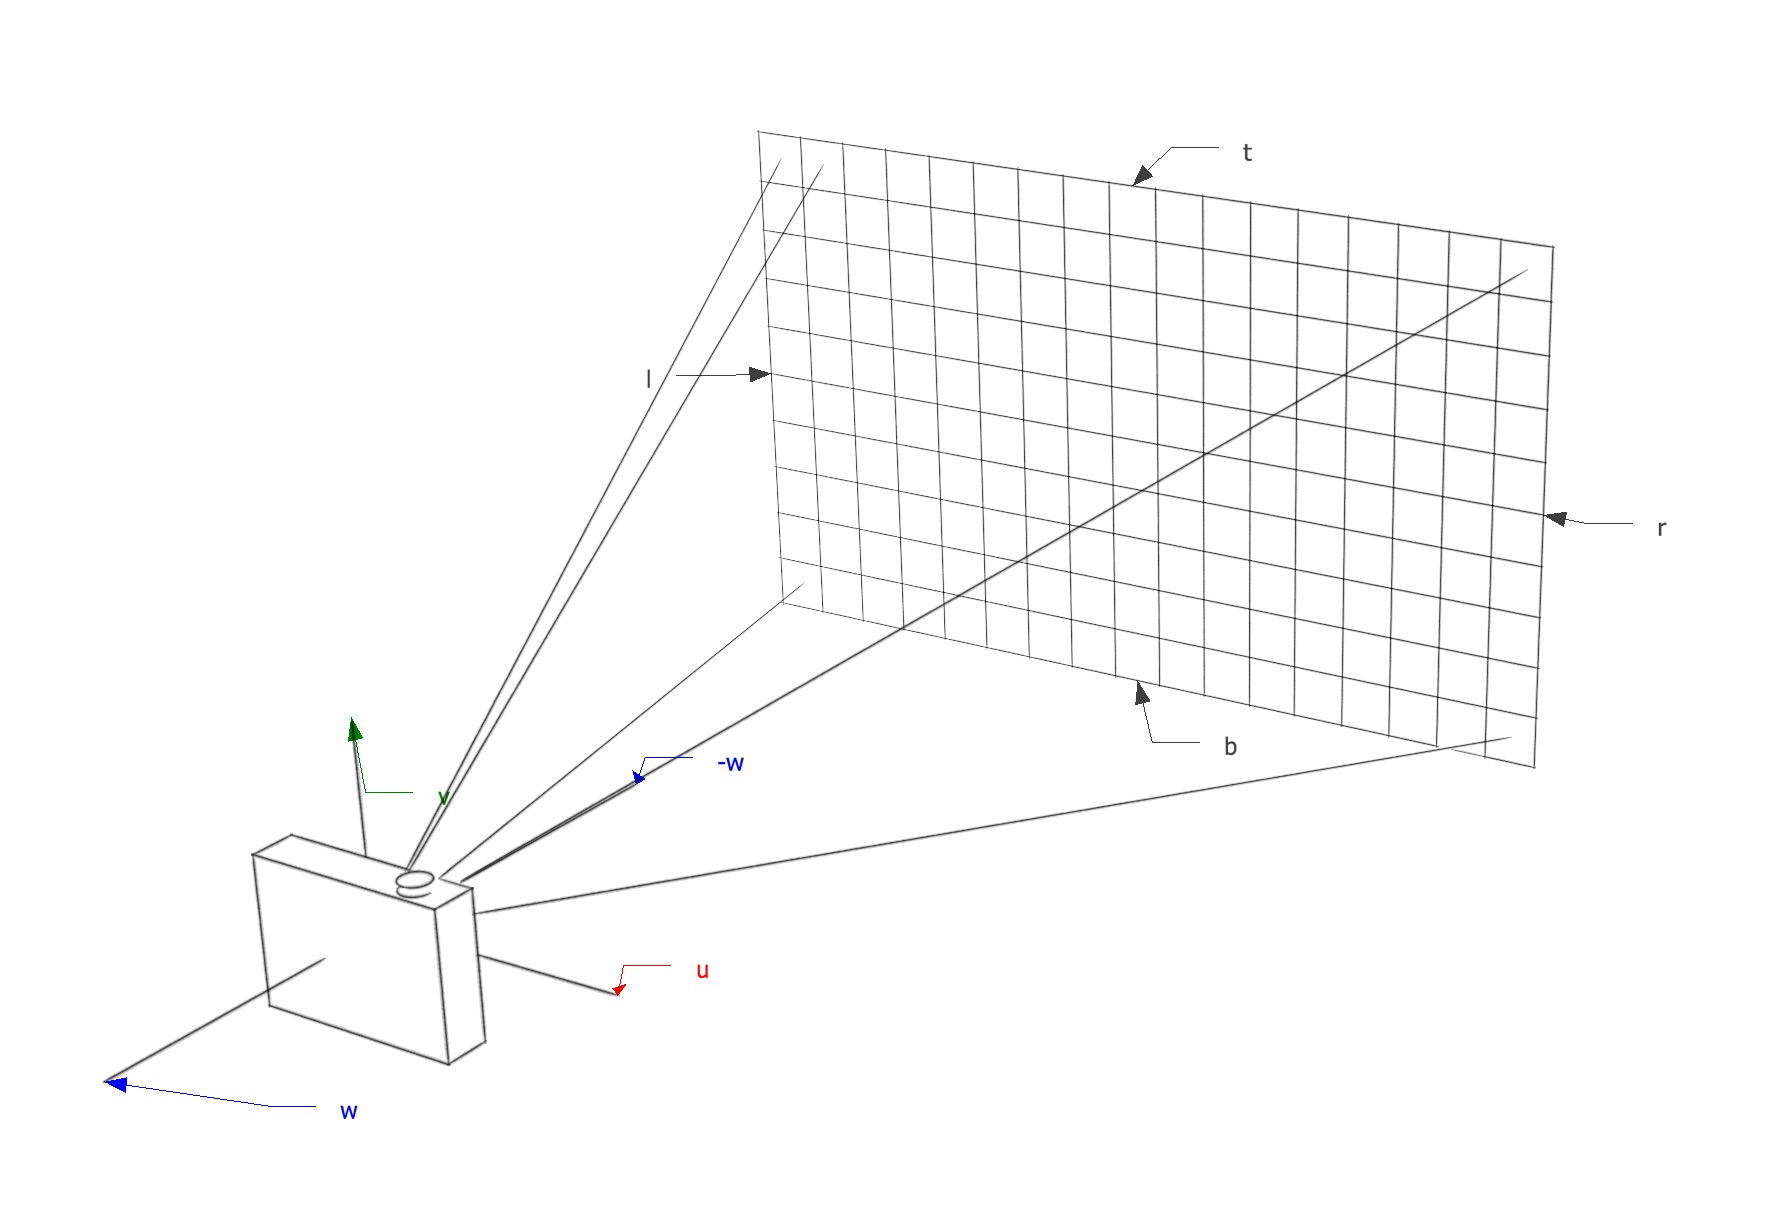
\includegraphics[scale=0.3]{raytracing_perspective}
	\caption{Перспективный вид}
	\label{fig:perspective_view}
\end{figure}
Соответственно необходимо корректировать вектор направления испускаемых лучей (см.~\ref{eq:ray_vector_eq}) следующим образом:
\begin{equation}
	D = -d\mathrm{w} + u\mathrm{n} + u\mathrm{v}
\end{equation}
где $u,v$ получены из расчета луча для каждого пикселя (см.~\ref{eq:pixel_rays}).
\begin{equation}
	\begin{aligned}
		u = l + (x + 0.5)\frac{r - l}{n_x}\\
		v = b + (y + 0.5)\frac{t - b}{n_y}
	\end{aligned}
	\label{eq:pixel_rays}
\end{equation}
В выражениях \ref{eq:pixel_rays} символы соответственно означают:
\begin{enumerate}
	\item $l,r$ - позиции левого  и правого краев изображения соответственно
	\item $t,b$ - позицции верхнего и нижнего краев изображения соответственно
	\item $x,y$ - координаты пикселя
	\item $n_x,n_y$ - количество пикселей по соответствующим осям изображения
\end{enumerate}
После выполненных преобразований будет получено представления луча, для которого будут вычисляться
пересечения с объектами.\cite{perspective_raytracing}

\section{Вывод}
В данном разделе был разобрана реализация выбранного алгоритма построения изображения, а также рассмотрены случаи поиска пересечений лучей  к конкретным примитивам.Была затронута 
тема построения перспективы для выбранного алгоритма и математическое обоснование его работы.














\begin{thebibliography}{9}
	\bibitem{Rodgers}
	Роджерс Д. Алгоритмические основы машинной графики. - 1-е изд. - Москва: Мир, 1989. - 512 с.
	\bibitem{global_model}
	Модель глобального освещения с трассировкой лучей [Электронный ресурс]. – Режим доступа: https://vunivere.ru/work71759/page3 (дата обращения 15.07.23)
	\bibitem{modern_ray_tracing}
	Современное состояние методов расчета глобальной освещенности в задачах реалистичной компьютерной графики [Электронный ресурс]. – Режим доступа: https://cyberleninka.ru/article/n/sovremennoe-sostoyanie-metodov-raschyota-globalnoy-osveschyonnosti-v-zadachah-realistichnoy-kompyuternoy-grafiki/viewer (дата обращения 15.07.23)
	\bibitem{SSR}
	Screen Space Reflection Techniques [Электронный ресурс]. – Режим доступа: https://ourspace.uregina.ca/handle/10294/9245 (дата обращения 15.07.23)
	\bibitem{reflexion_types}
	Отражение в играх. Как работают, различия и развитие технологий [Электронный ресурс]. – Режим доступа: https://clck.ru/34zZCf (дата обращения 15.07.23)
	\bibitem{simple_reflexion_types}
	Простые модели освещения  [Электронный ресурс]. – Режим доступа: https://grafika.me/node/344 (дата обращения 15.07.23)
	\bibitem{primitives_raytracing_equations}
	Ray tracing primitives  [Электронный ресурс]. – Режим доступа: https://www.cl.cam.ac.uk/teaching/1999/AGraphHCI/SMAG/node2.html (дата обращения 20.07.23)
	\bibitem{perspective_raytracing}
	Ray tracing  [Электронный ресурс]. – Режим доступа: https://www.mauriciopoppe.com/notes/computer-graphics/ray-tracing/ (дата обращения 23.07.23)


\end{thebibliography}

\addcontentsline{toc}{chapter}{Список литературы}



\end{document}